%%%%%%%%%%%%%%%%%%%%%%%%%%%%%%%%%%%%%%%%%%%%%%%%%%%%%%%%%%%%%%%%%%%%%%%%%%%%%%%%
%2345678901234567890123456789012345678901234567890123456789012345678901234567890
%        1         2         3         4         5         6         7         8

\documentclass[letterpaper, 10 pt, conference]{ieeeconf}  % Comment this line out
                                                          % if you need a4paper
%\documentclass[a4paper, 10pt, conference]{ieeeconf}      % Use this line for a4
                                                          % paper

\IEEEoverridecommandlockouts                              % This command is only
                                                          % needed if you want to
                                                          % use the \thanks command
\overrideIEEEmargins
% See the \addtolength command later in the file to balance the column lengths
% on the last page of the document
\usepackage{graphicx}
\usepackage{url}
\urlstyle{same}

% The following packages can be found on http:\\www.ctan.org
%\usepackage{graphics} % for pdf, bitmapped graphics files
%\usepackage{epsfig} % for postscript graphics files
%\usepackage{mathptmx} % assumes new font selection scheme installed
%\usepackage{times} % assumes new font selection scheme installed
%\usepackage{amsmath} % assumes amsmath package installed
%\usepackage{amssymb}  % assumes amsmath package installed

\title{\LARGE \bf
An Empirical Study on the Use and Effectiveness of the Unified Modeling Language in the California Software Industry*
}

%\author{ \parbox{3 in}{\centering Huibert Kwakernaak*
%         \thanks{*Use the $\backslash$thanks command to put information here}\\
%         Faculty of Electrical Engineering, Mathematics and Computer Science\\
%         University of Twente\\
%         7500 AE Enschede, The Netherlands\\
%         {\tt\small h.kwakernaak@autsubmit.com}}
%         \hspace*{ 0.5 in}
%         \parbox{3 in}{ \centering Pradeep Misra**
%         \thanks{**The footnote marks may be inserted manually}\\
%        Department of Electrical Engineering \\
%         Wright State University\\
%         Dayton, OH 45435, USA\\
%         {\tt\small pmisra@cs.wright.edu}}
%}

\author{Jacob Nogle$^{1}$ and Dr. Bruno C. da Silva$^{2}$% <-this % stops a space
\thanks{*This work was produced as a student senior project at Cal Poly, San Luis Obispo}% <-this % stops a space
\thanks{$^{1}$J. Nogle is an undergraduate 	student at Cal Poly, San Luis Obispo in the department of Computer Science and Software Engineering}%
\thanks{$^{2}$Dr. Bruno C. da Silva is a member of the Department of Computer Science and Software Engineering faculty at Cal Poly, San Luis Obispo, and the advisor of this project}%
}


\begin{document}



\maketitle
\thispagestyle{empty}
\pagestyle{empty}


%%%%%%%%%%%%%%%%%%%%%%%%%%%%%%%%%%%%%%%%%%%%%%%%%%%%%%%%%%%%%%%%%%%%%%%%%%%%%%%%
\begin{abstract}

The Unified Modeling Language (UML) has been the ``de facto" standard for modeling in all phases of the software development life-cycle for many years now. Many studies have been conducted to examine the use and effectiveness as well as the overall perception of UML in Software Engineering. Based on these studies, the cost effectiveness of using UML in modeling has not consistently been shown to be worth the effort. This study aims to examine these same topics with an emphasis on specific geographic location, as well as project domain in order to search for more consistent results on UML use and opinion on cost-effectiveness.

\end{abstract}

%%%%%%%%%%%%%%%%%%%%%%%%%%%%%%%%%%%%%%%%%%%%%%%%%%%%%%%%%%%%%%%%%%%%%%%%%%%%%%%%
\section{INTRODUCTION}

In Software Engineering, the software development life-cycle goes far beyond writing code and testing it. The birth of a software product begins with rigorous analysis of customer needs, requirements, and architectural design. One of the most prominent tools in this phase of the software development life-cycle is the Unified Modeling Language (UML), ``a family of graphical notations, backed by single meta-model, that help in describing and designing software systems, particularly software systems built using the object-oriented (OO) style'' \cite{fowler}. UML is used for modeling many aspects of a software product on many different levels, from use cases to architecture, and more.  But despite being so widely used in both the enterprise and education, there seem to be doubts regarding the applicability and effectiveness of UML in software development. Many studies have been conducted on this issue and have not been able to produce consistent results on whether or not UML benefits software development \cite{c2}.

For software engineers in industry, it is important to find an answer to this question of UML applicability in order to maximize their productivity and not waste time on modeling if it is proven to be not cost-effective. One strategy that has been employed by researchers in an attempt to produce more consistent results and compliment existing work is reducing the targets of their research to a specific geographic location. We employed this strategy in our study by reducing our target demographic to a single state in the U.S. In addition, we placed a focus on participant project domain to examine the effect this factor had on UML use and perception.

Our study was centered around the following research questions:

\begin{description}
  \item $\ast$ \textbf{RQ1: What is the frequency of UML use in practice?}
  \item $\ast$ \textbf{RQ2: What are the benefits of using UML?}
  \item $\ast$ \textbf{RQ3: What is the diffusion of UML use throughout the development process?}
  \item $\ast$ \textbf{RQ4: What are the main issues that hinder the UML use in practice?}
  \item $\ast$ \textbf{RQ5: What improvements can be done to increase the UML use?}
  \item $\ast$ \textbf{RQ6: Does project domain influence the use of UML modeling practices?}
  \item $\ast$ \textbf{RQ7: Does geographic region influence the use of UML modeling practices?}
\end{description}
\  \\
The remainder of the paper is organized into four sections: 
\begin{description}
  \item $\cdot$ Section 2: Related Works
  \item $\cdot$ Section 3: Survey Design
  \item $\cdot$ Section 4: Results and Discussion
  \item $\cdot$ Section 5: Conclusion
\end{description}

\section{RELATED WORKS}

The most closely related work and the true inspiration of this study is a similar  study conducted by Dr. Bruno da Silva et al. on the UML use in the Brazilian software industry \cite{c3}. The authors of the location-specific study concluded that ``the UML is not often used in the work life of participants. In addition,
no relationship was identified between the use of UML and the participant company being a software factory." Because this study was able to produce consistent results, it prompted us to limit our participants to an isolated geographic region. 

Other researchers have tried to narrow the scope of their studies and produce more consistent results by limiting their examination to a single domain. For example, a study by Ho-Quan et al. examines the use and perception of UML specifically in open source projects \cite{c6}. Their research concluded that UML ``helps new contributors and is generally perceived as supportive", but also does not tend to attract new contributors. They also found that collaboration seemed to be the most important motivation for using it. We thought that examining the influence of project domain on UML use and effectiveness would be a factor of interest, and made sure to include questions on our survey about the domain participants were working in.

There have been a number of other notable works produced on the subject of UML use and effectiveness that have taken a broader approach without focusing on a single geographic location or domain. Although these studies offer great insight into the Software Engineering industry as a whole, they have struggled to produce as consistent results giving proof to the effectiveness or ineffectiveness of using UML. Harald Störrle's survey on how conceptual models are used in software development came to conclusions that both contrast and complement existing studies on the topic, but offers explanations for these contradictions, which include cultural differences in modeling that we aimed to explore in our own research \cite{c5}. Nugroho and Chaudron conducted a study on UML use and perceived impact whose most important conclusion was that ``the impact of using the UML on productivity is perceived mostly in the design, analysis, and implementation phases" \cite{c4}. Finally, Chaudron, Nugroho, and Heijstek examined empirical evidence regarding the costs and benefits of using UML, concluding that the industrial practice of software modeling using UML is very diverse, and little evidence has been collected on either the effectiveness or ineffectiveness of modeling, as it is difficult to quantify \cite{c7}.

\section{Survey Design}

In order to collect data on the use and effectiveness of UML for the study, we reached out to as many professionals who work in the software industry by means of an online survey created using Google Forms, with a total of 34 questions. It was a goal to include questions addressing each and every one of our research questions, although it wasn't completely balanced, being that certain research questions held a heavier weight than others. 10 questions were used for demographic purposes including location and opinion on UML cost effectiveness, 3 questions pertaining to domain, 4 questions pertaining to frequency of UML use, 4 questions pertaining to hindrances to UML use, 1 question related to the diffusion of UML use throughout the development process, 5 questions related to the benefits of using UML, and 2 questions related to improvements that can be done to increase UML usage. The remaining 5 questions were asking for additional information about the participants, comments about the survey, and whether or not they were interested in receiving the results. Out of the 34 questions, 11 were open questions. The rest were either multiple choice, checkbox, Likert scale, or multiple choice grid questions. The survey was split up into seven sections or groupings of questions which all related to a different topic or focus. There were a number of questions that would have been nice to analyze but ultimately we had to cut out in order to minimize the survey completion time, including questions on others forms of modeling besides UML and the three different ways of using UML outlined in \cite{fowler}.

Our only criteria for a qualifying participant in the survey were that they currently were working in the US state of California (our isolated geographic region), knew what UML was, and had used UML in some way in their current organization. If a participant answered a question that disqualified them from our target demographic, they were sent to the end of the survey and thanked for their participation, with an opportunity to provide feedback on the parts of the survey they had access to. There were multiple avenues that were utilized in order to advertise the survey. First, we reached out to all of the professionals in the California software industry that we were already acquainted with and were confident would help us out by completing the survey. Second, we used various online communities that we knew many developers would be members of. These included LinkedIn groups specific to certain programming languages and Software Engineering methodologies, subreddit pages with Software Engineering-related topics, and Slack channels focused on iOS and Android development. The survey released to the aforementioned individuals can be viewed in its entirety through an archival link in the References section\cite{c8} Finally, we released the survey to a group of Software Engineering graduate students at Cal Poly that had held internships in the software industry before. For the student respondents, we modified the phrasing of most of the survey questions to ask about their internship--rather than full-time professional--experience. This modified version of the full survey can also be found in the References section\cite{c9}. To encourage individuals in participating in our survey, we offered a \$10 Amazon.com gift card for all participants who met our target demographic and completed the entirety of the survey. 

\section{RESULTS AND DISCUSSION}

Our survey received a total of 115 responses from the various avenues we explored in advertising it. However, because we decided to offer a reward for completing our survey, we ran into the issue of falsified/repeated responses (mainly from Reddit). We reserved the right to remove any responses suspected of falsified or repeated answers from previous responses. Unfortunately in the end we had to remove approximately 64 responses for these violations, leaving us with 51 legitimate participants. Out of these 51 participants, only 23 met our target demographic of knowing what UML was, having utilized it in real-world software development projects, and working in California, USA. Out of the 51 total respondents, only 3 were eliminated for not knowing what UML was (5.9\%). 13 knew what UML was but had never utilized it in in real-world software projects (25.5\%). The remaining 12 disqualified were done so because of their current work location not being California (23.5\%). Although the number of remaining responses was less than ideal, it was important to analyze this data to hopefully catalyze further location-specific Software Engineering research, and get an idea of the relative state of UML use and effectiveness in California to be expanded upon in later studies. The following subsections will first explore the respondent demographics, and then revisit each individual research question outlined in the introduction, displaying the most important findings in the survey data relating to each one.

\subsection{Respondent Demographics}

Figures 1-4 show the demographics of our 23 qualified respondents. Of these 23 individuals, 20 (87\%) identified as male and only 3 (13\%) as female. Over 80\% of respondents (19 out of 23) were under the age of 35. 
The majority of respondents' educational background was a Bachelor's Degree (65.2\%). Work experience was the most balanced, with the most respondents (7) having 10+ years of experience (30.4\%), but the remaining respondents (16) were reasonably varied across the five other categories.

	\begin{figure}[!htb]
      \centering
      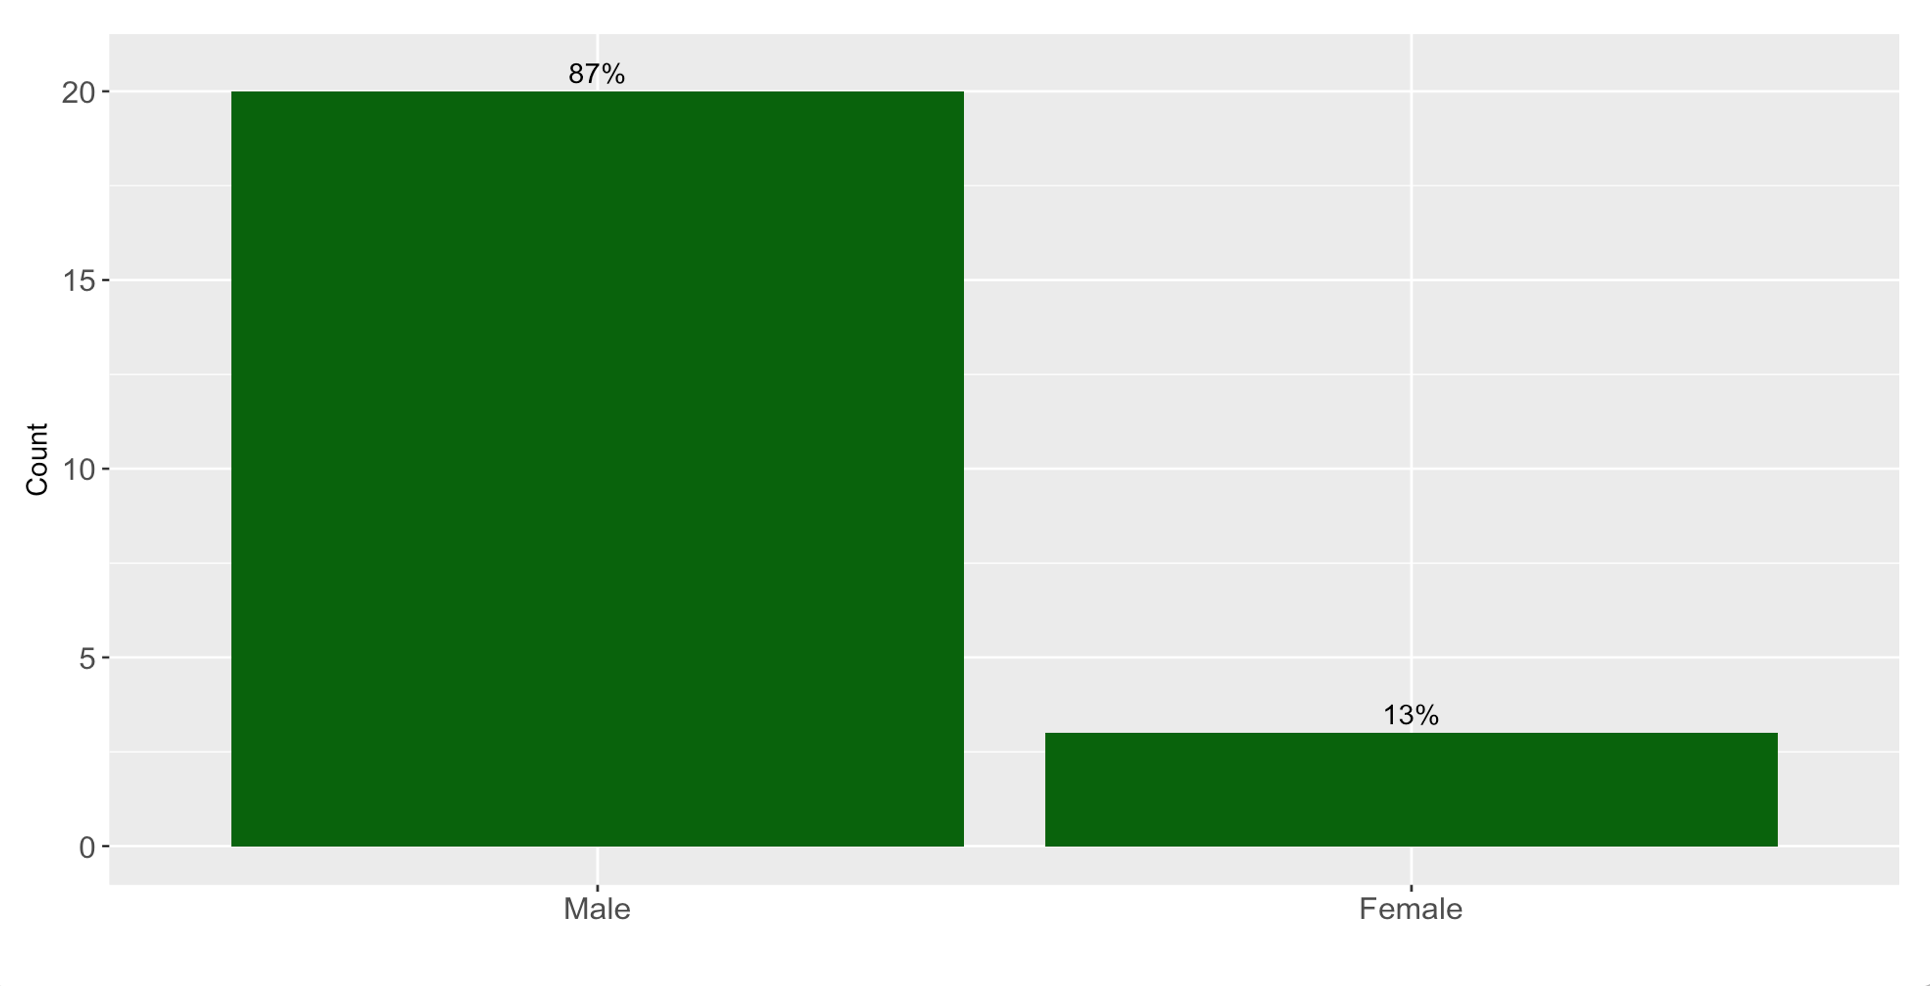
\includegraphics[scale=0.25]{Plots/GenderPlot}
      \caption{Gender distribution of qualified participants}
      \label{GenderPlot}
   \end{figure}
   
   \begin{figure}[!htb]
      \centering
      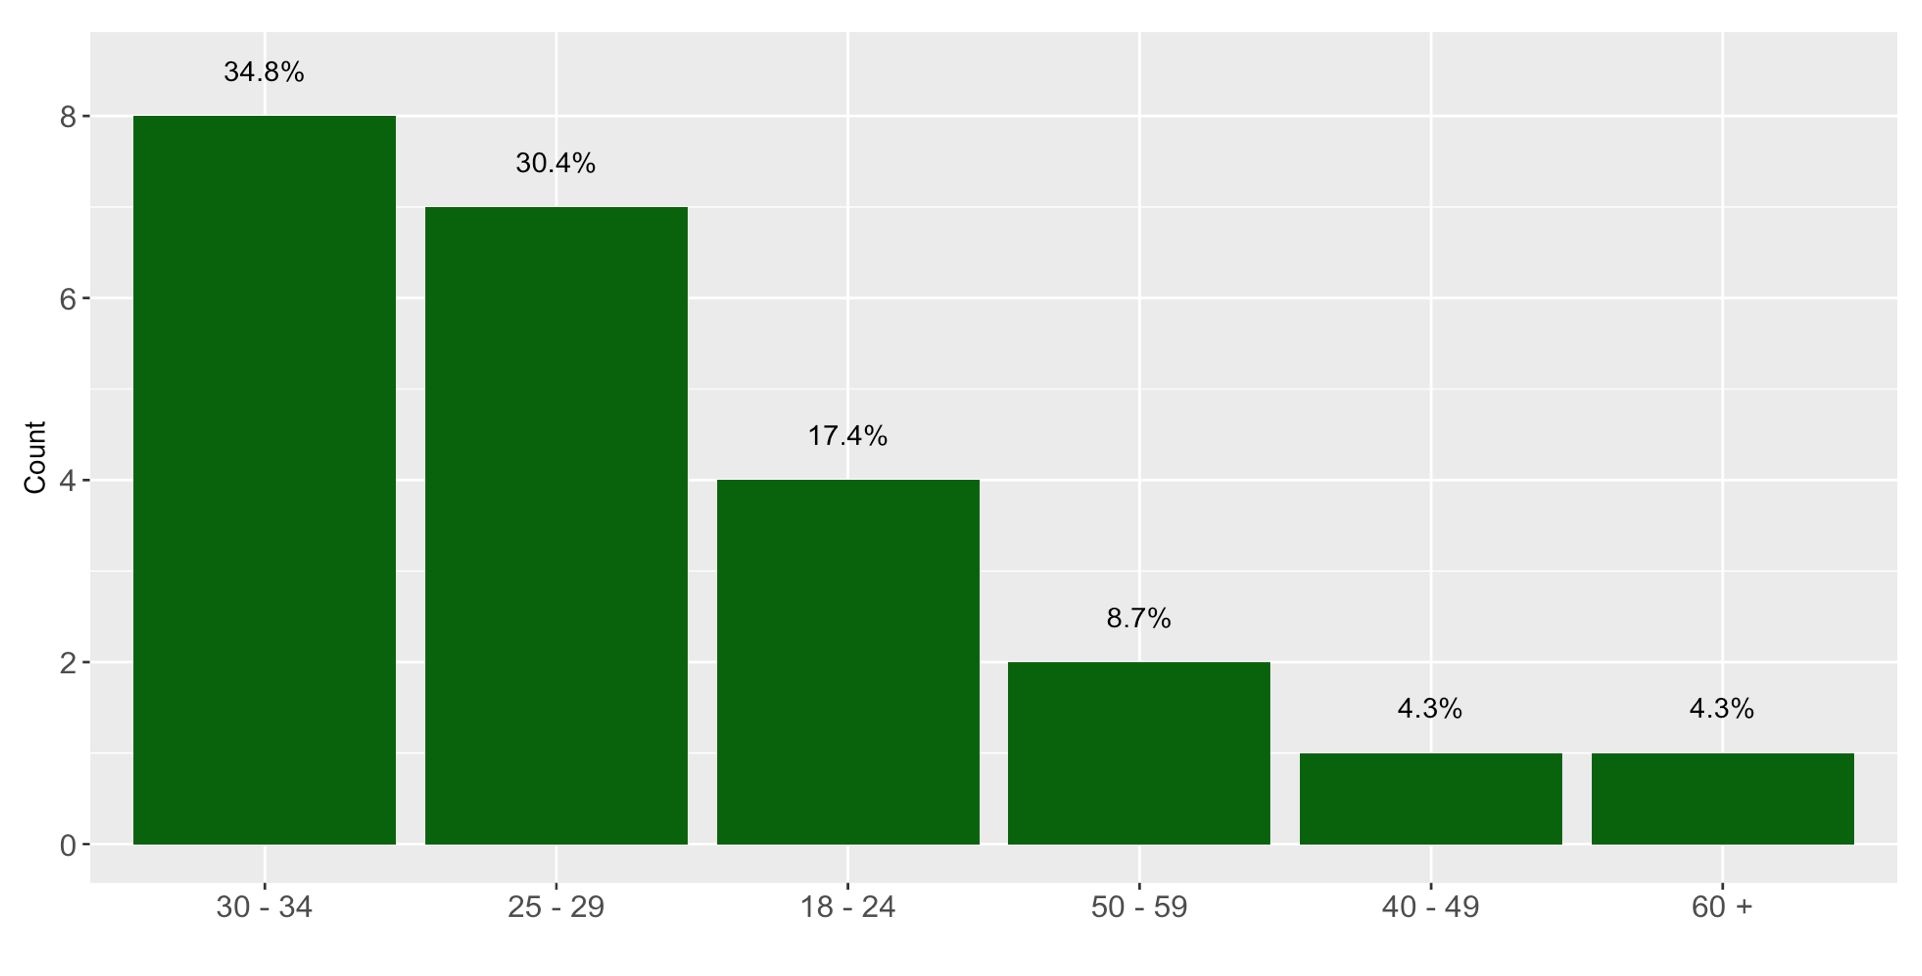
\includegraphics[scale=0.25]{Plots/AgePlot}
      \caption{Age distribution of qualified participants}
      \label{AgePlot}
   \end{figure}
   
   \begin{figure}[!htb]
      \centering
      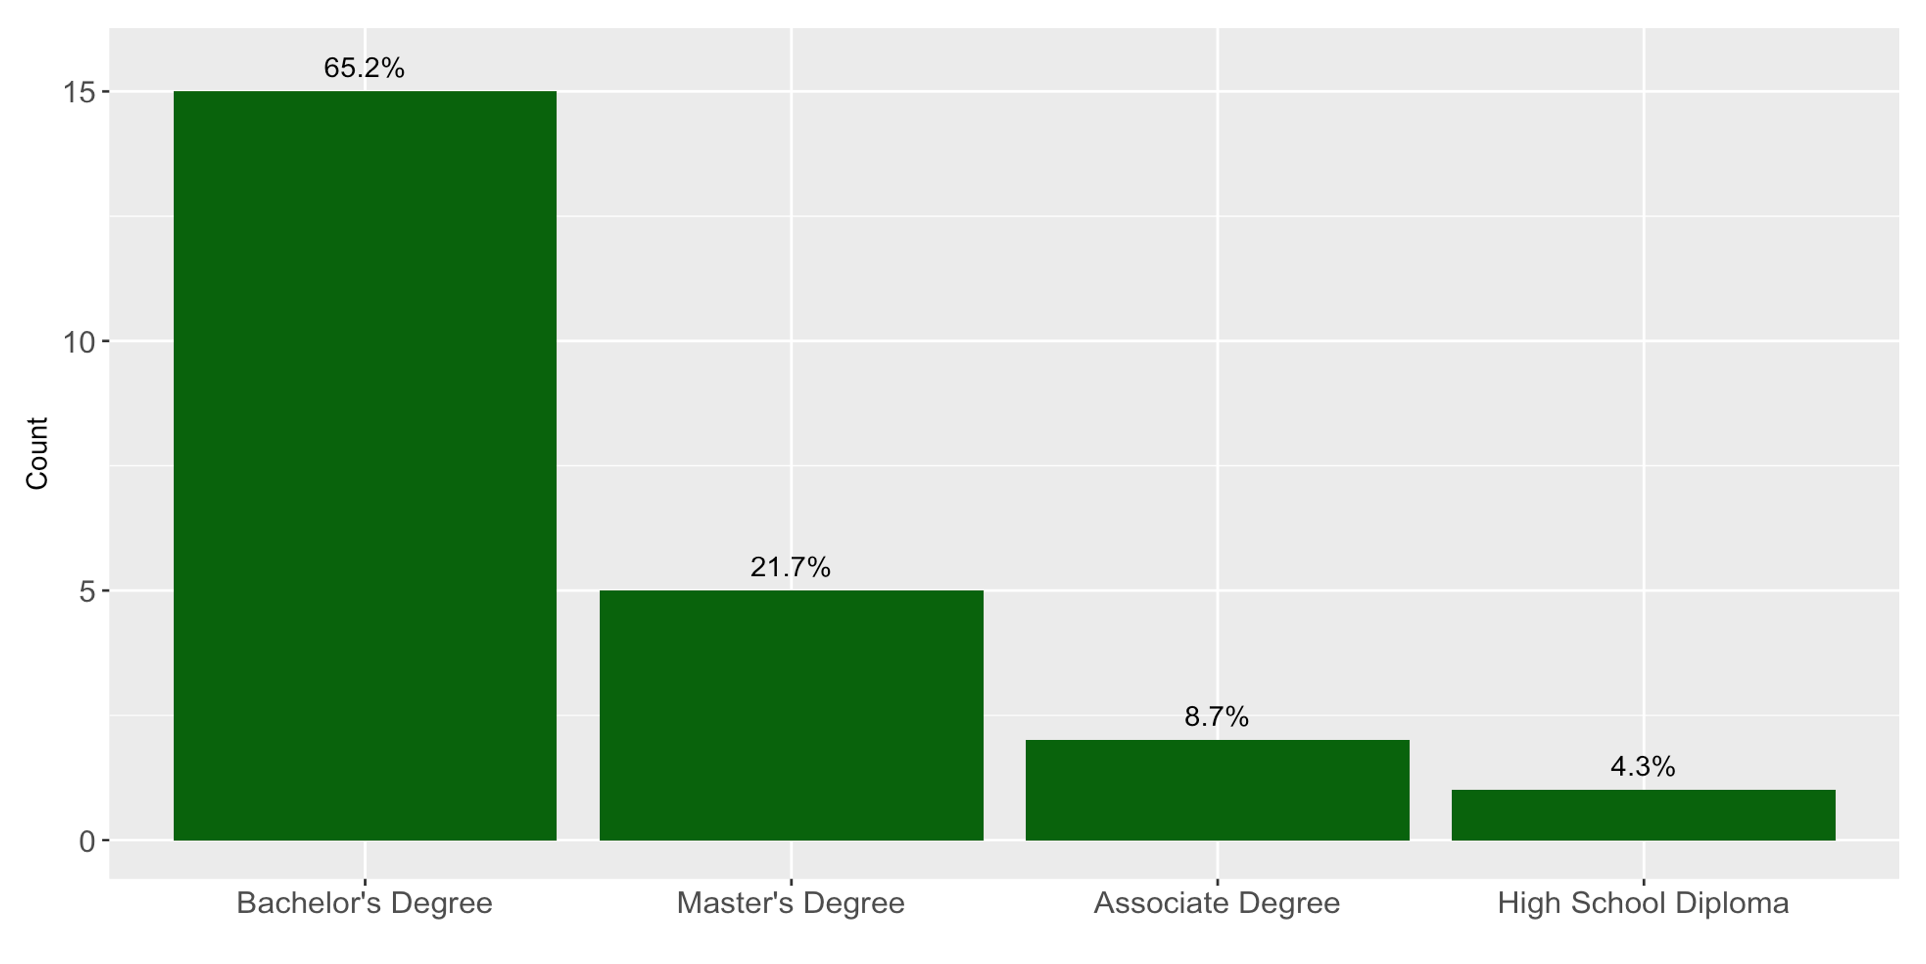
\includegraphics[scale=0.25]{Plots/EducationPlot}
      \caption{Education distribution of qualified participants}
      \label{EducationPlot}
   \end{figure}
   
   \begin{figure}[!htb]
      \centering
      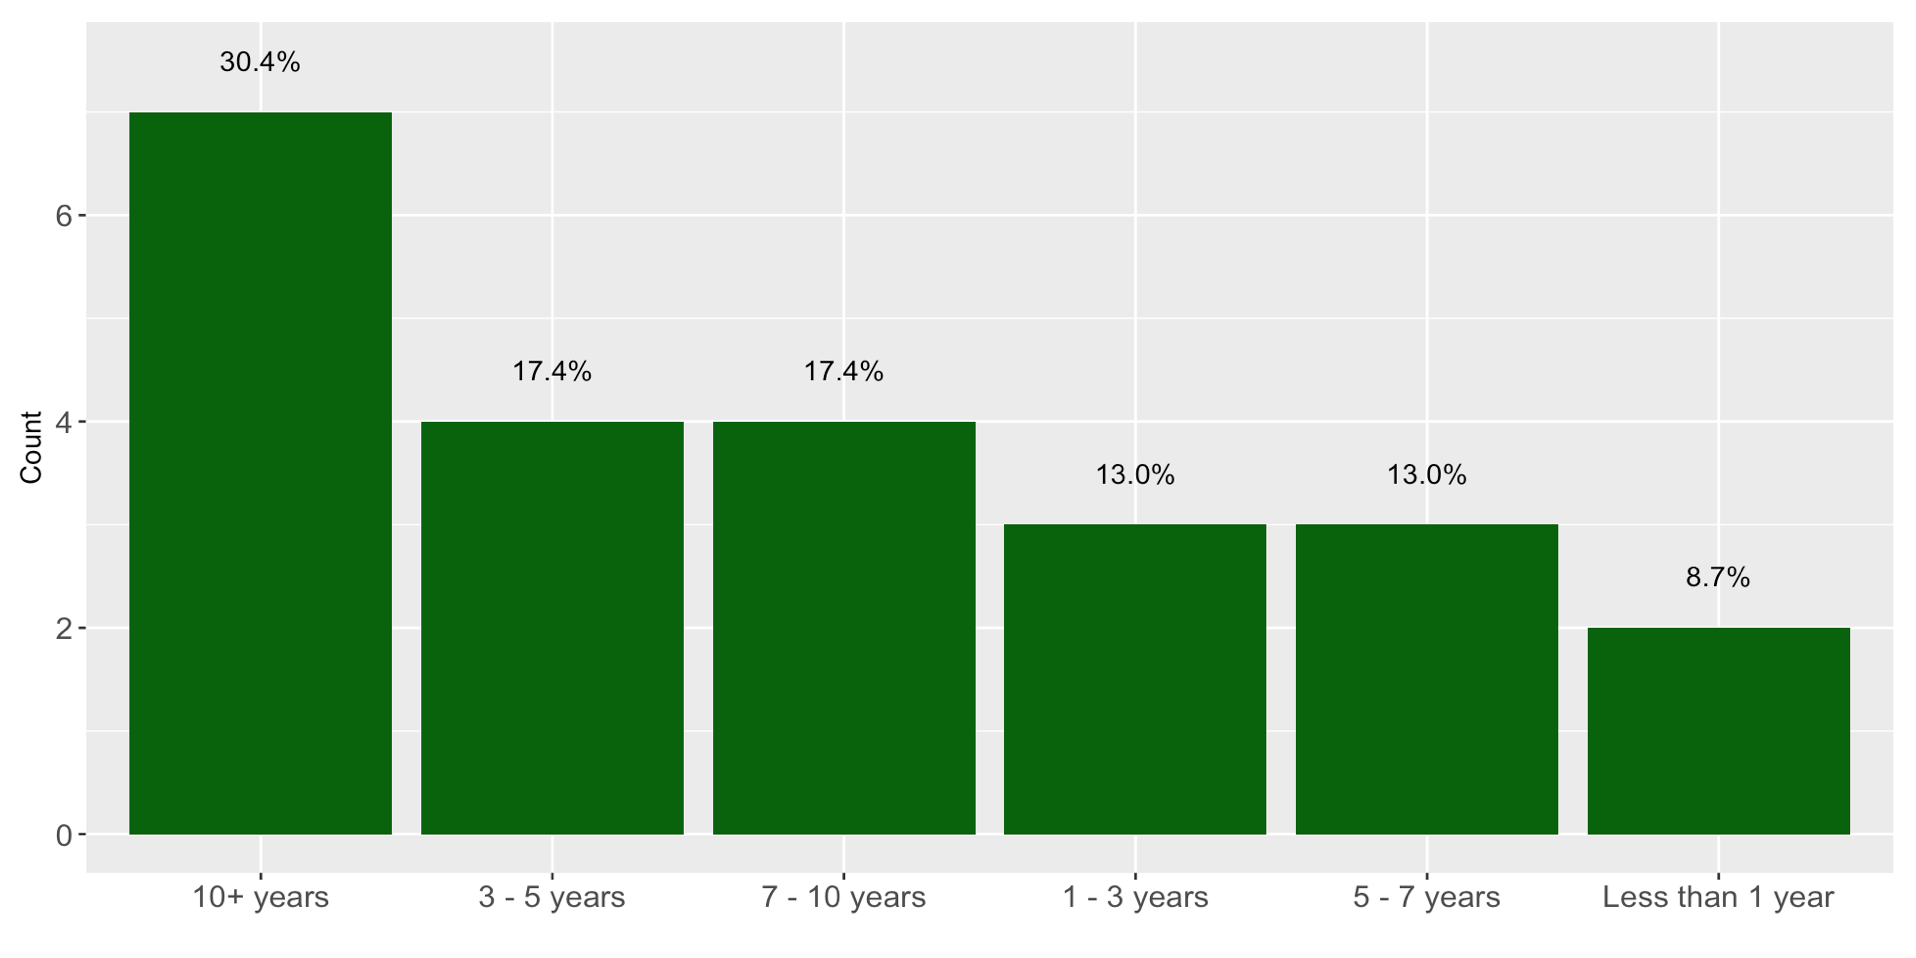
\includegraphics[scale=0.25]{Plots/WorkExperiencePlot}
      \caption{Work Experience distribution of qualified participants}
      \label{WEPlot}
   \end{figure}
   
   
\subsection{RQ1: What is the frequency of UML use in practice?}

To address this first research question, we took two main approaches in our survey to explore the frequency of UML use of our respondents. First, we simply asked ``Of the projects you've participated in at your current organization, for how many of those have you utilized UML for any purpose in your software development work?", allowing the respondents to answer with a range of percentages of the projects they have used UML in any way (\textless 10\%, 10-50\%, 51-90\%, or 91-100\%). Figure 5 details the responses to this question, with the majority of participants (16 out of 23) answering that they used UML in either 10-50\% or 51-90\% of their projects.

The second approach we took was to ask participants specifically which UML diagrams they used in their work, and how often. We split UML diagrams into the categories of structural UML diagrams (Class, Object, Component, Composite Structure, Deployment) and behavioral UML diagrams (Activity, Sequence, Use Case, State, Communication, Interaction Overview, Timing) and asked how often (Never, Rarely, Sometimes, Often, Usually, or Always) they used each diagram in their software development work at their current organization. Figures 6 and 7 show the results of these questions. For structural UML diagrams, the most commonly reported diagram used was the Class Diagram, with no respondents answering that they had never used one in their work. For all other structural UML diagrams, the most common answer was that respondents had never used them in their work. For behavioral UML diagrams, the most common answer for each diagram was that respondents had never used these diagrams, save the State Diagram, where the most common answer was ``Sometimes" and ``Often".
	
    \begin{figure}[!htb]
      \centering
      \framebox{\parbox{3in}{\textbf{Conclusion of RQ1: } Average UML use for any purpose in software development work for is not extremely high nor extremely low (top or bottom tenth percentile), but falls somewhere in between 10-90\%. Additionally, this UML use is not evenly distributed across different UML diagrams. Certain diagrams are used much more often than others.
}}
      \label{RQ1Concl}
   \end{figure}
   
	\begin{figure}[!htb]
      \centering
      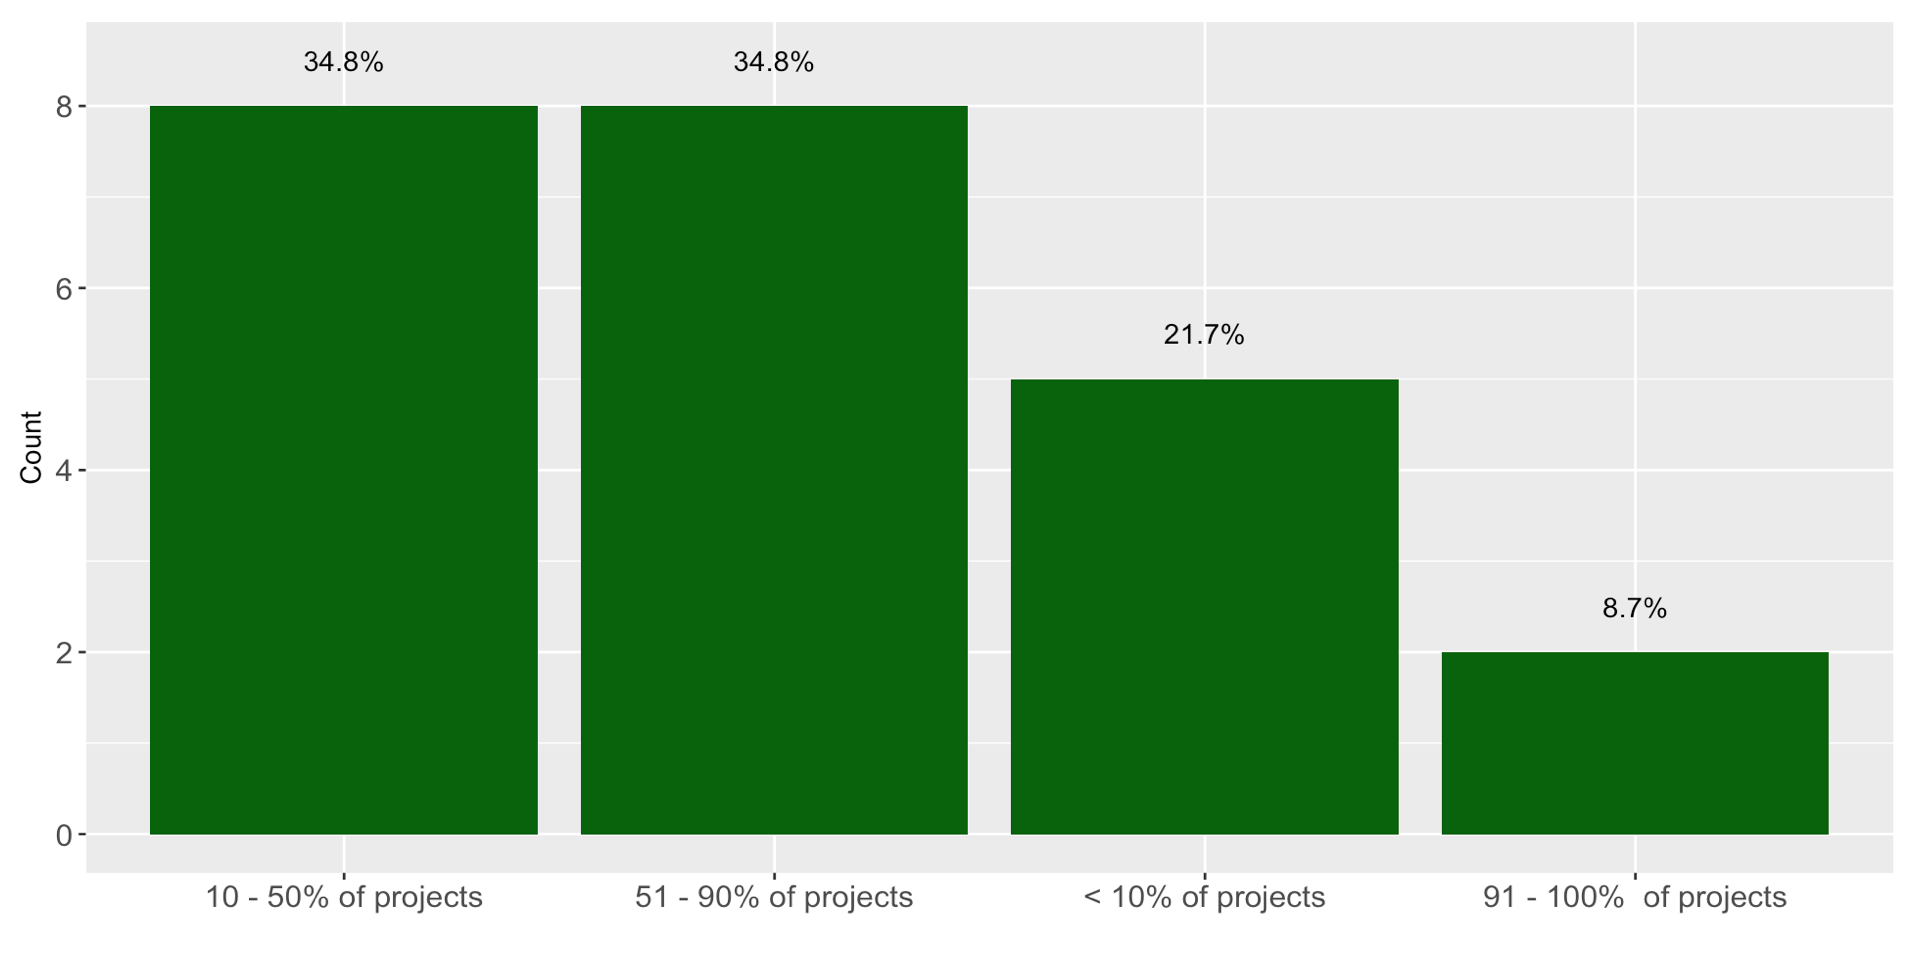
\includegraphics[scale=0.25]{Plots/GenUmlUsePlot}
      \caption{General frequency of UML use distribution}
      \label{GenUML}
   \end{figure}
   
   \begin{figure}[!htb]
      \centering
      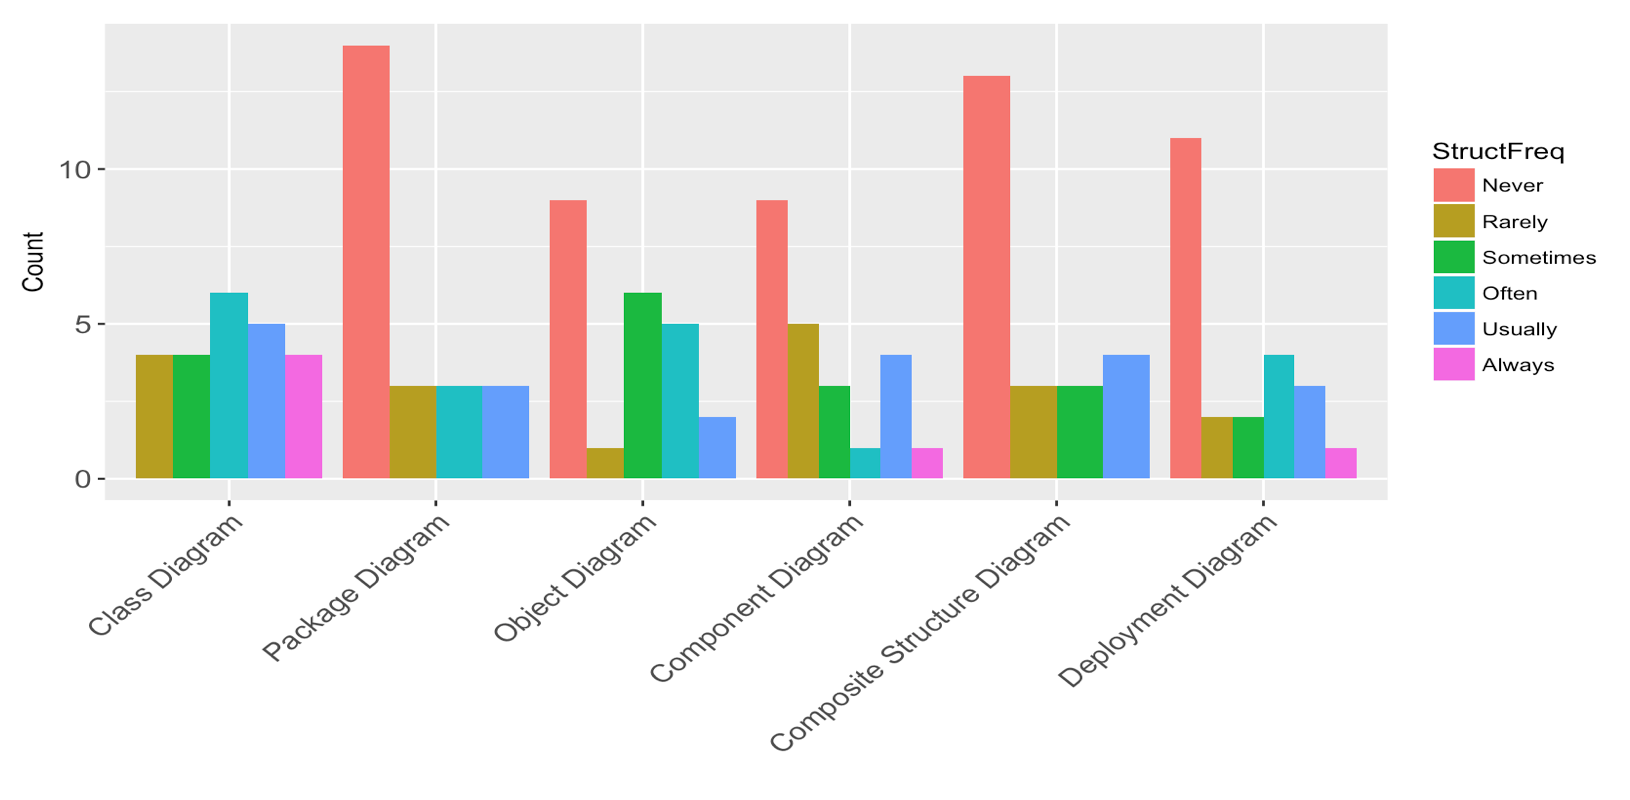
\includegraphics[scale=0.3]{Plots/StructUMLPlot}
      \caption{Frequency of structural UML diagram use}
      \label{StructUML}
   \end{figure}
   
   \begin{figure}[!htb]
      \centering
      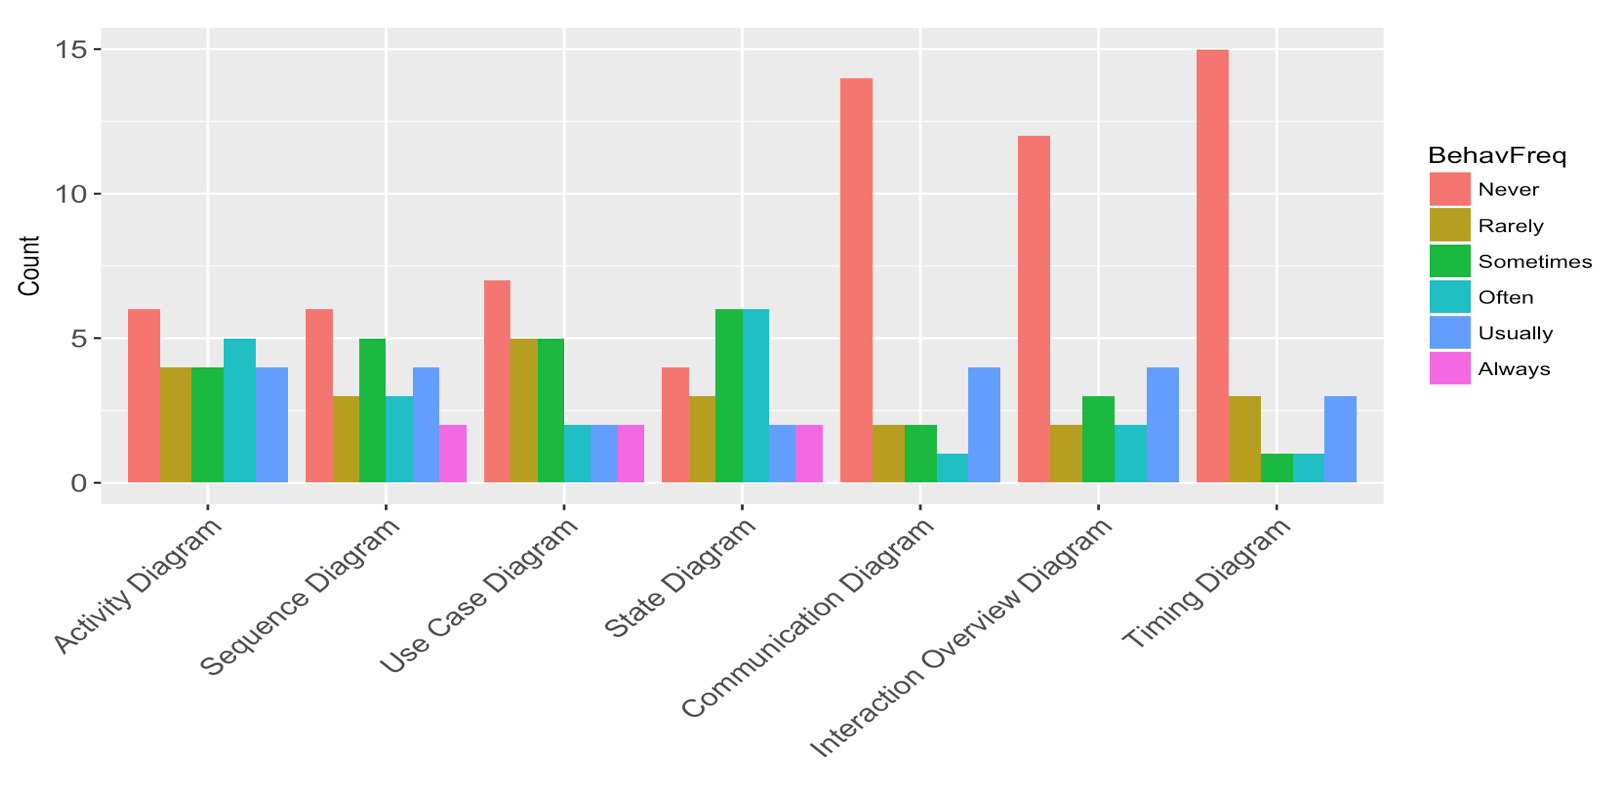
\includegraphics[scale=0.3]{Plots/BehavUMLPlot}
      \caption{Frequency of behavioral UML diagram use}
      \label{BehavUML}
   \end{figure}

\subsection{RQ2: What are the benefits of using UML?}

To analyze the opinions of respondents pertaining to this research question, we posed an open question simply asking ``In your opinion, what are the biggest benefits of using UML in software development?", and coded the respondents' answers manually. Based on the responses, we came up with 8 different codings for the benefits of using UML: 1 - Increased Efficiency, 2 - Better Communication, 3 - Helps Approach Coding, 4 - Better Results, 5 - Explain Complexities, 6 - Visualization, 7 - Find Problems Easier, 8 - Common Notation. Figure 8 shows the results of this question. The top three most common responses were 2 - Better Communication (33.3\%), 1 - Increased Efficiency (16.7\%), as well as 5 - Explain Complexities and 8 - Common Notation both with 12.5\% of responses.

In addition to this open question on the benefits of UML use, we also asked a series of four questions answered using a Likert Scale from 0 to 5 on the opinions of how UML use is related to specific benefits. We asked ``To what extent does UML modeling reduce the effort in writing/debugging code?", ``To what extent does UML modeling increase productivity in delivering software?", ``To what extent does UML modeling increase the quality of the software being developed/delivered?", and ``To what extent does UML modeling increase communication effectiveness within teams?". The results of these questions (based on the Likert Scale) can be visualized in Figure 9. For the question regarding UML's influence on the effort in coding and debugging, the trend was that more respondents answered that UML does in fact reduce the effort in coding/debugging, but not to an extreme level (34.8\% of respondents chose a 4 on the Likert Scale). For UML's influence on productivity, the most respondents (30.4\%) chose a 2 on the Likert Scale, meaning they did not see UML affecting productivity in a positive way. For UML's influence on software quality, 63.6\% of respondents chose either a 3 or 4 on the Likert Scale, implying UML has a slight positive effect. Finally, 81.8\% of respondents chose a 3, 4, or 5 on the Likert Scale for UML increasing communication effectiveness in software teams.

	\begin{figure}[!htb]
      \centering
      \framebox{\parbox{3in}{\textbf{Conclusion of RQ2: } The most common perceived benefit of using UML in software development for our respondents is for communication purposes. Other notable benefits include increased efficiency, reducing complexities, and having a common notation. UML seems to have at least a slight positive effect on the effort required in coding/debugging as well as on software quality for our respondents, but not necessarily on productivity in delivering that software. 
}}
      \label{RQ2Concl}
   \end{figure}
   
	\begin{figure}[!htb]
      \centering
      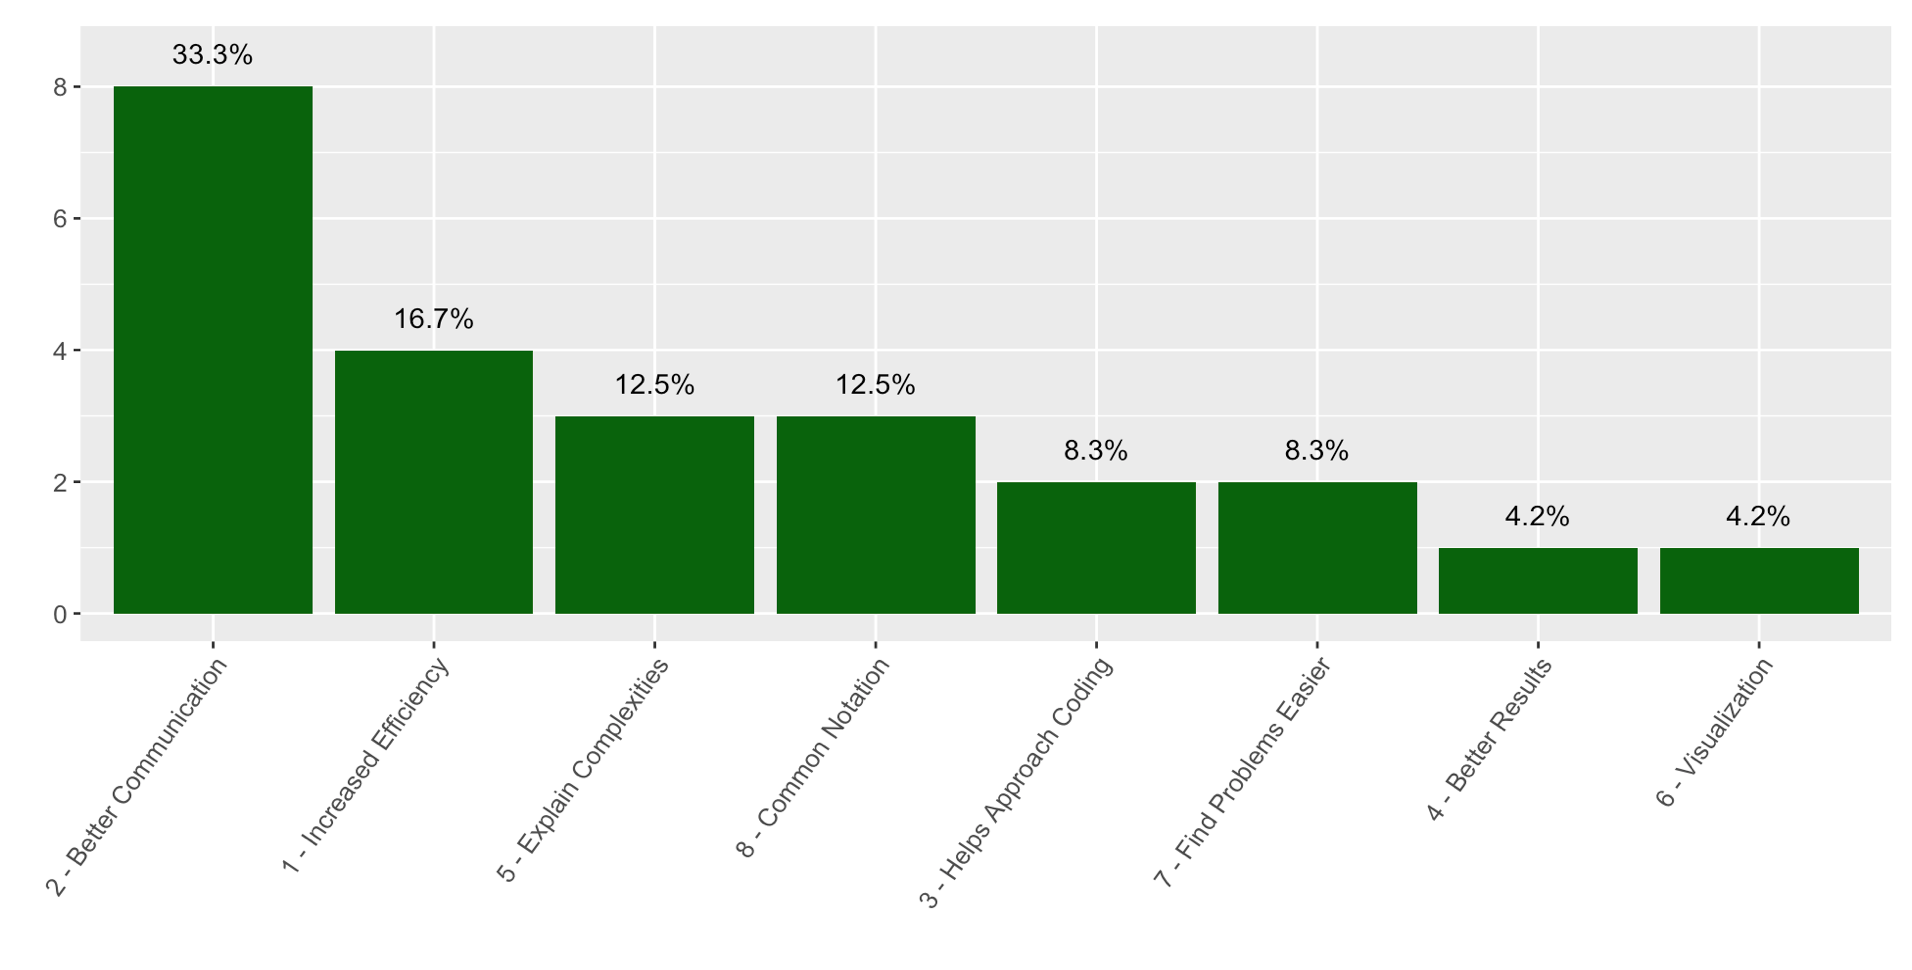
\includegraphics[scale=0.25]{Plots/BenefitsPlot}
      \caption{Respondent opinion on the benefits of UML usage}
      \label{BenefitsUML}
   \end{figure}
   
   \begin{figure}[!htb]
      \centering
      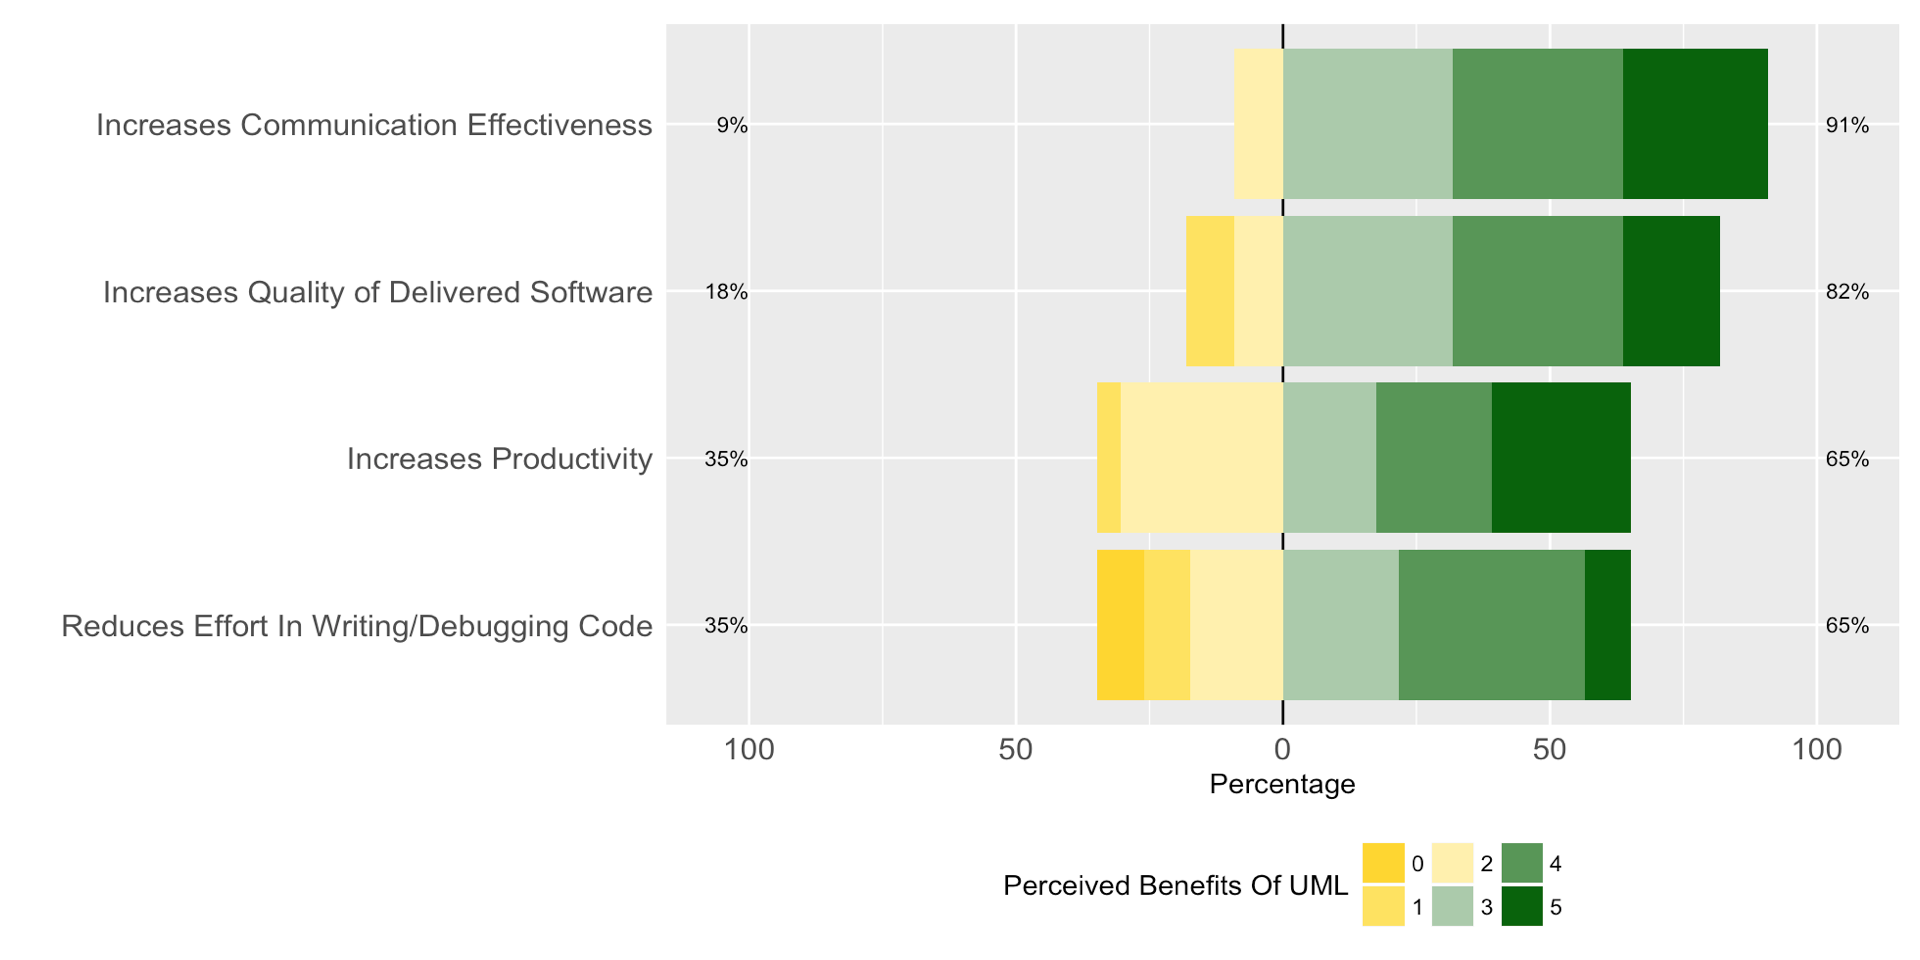
\includegraphics[scale=0.25]{Plots/LikertPlot.png}
      \caption{Scaled respondent opinion on specific benefits of UML usage}
      \label{OpCodeUML}
   \end{figure}
   
\subsection{RQ3: What is the diffusion of UML use throughout the development process?}

This research question was one of the more difficult ones to measure directly. In order to speculate, the question we asked was ``For what activities do you use UML in your software development work at your current organization? We chose to let this question be an open question, since we imagined that we could not possibly cover all the possible activities in the software development life-cycle, and individuals might prefer to word these activities differently, although they mean the same thing. Figure 10 displays the responses for this open questions, which we coded into 8 categories: 1 - Modeling, 2 - Communication, 3 - Documentation, 4 - Understanding Requirements, 5 - Design, 6 - Comprehending Overall Picture, 7 - Research, 8 - Presenting. The responses were generally balanced, with 6 of the 8 categories receiving over 10\% of the responses. 1 - Modeling and 5 - Design were the most common responses, both at 19.2\%. 3 - Documentation and 8 - Presenting were the second most common at 15.4\%. 2 - Communication and 4 - Understanding Requirements were the third most common at 11.5\%. Based on these responses, we found UML is used by respondents for a variety of activities in the software development life-cycle. Among the most common of these activities are modeling, design, documentation, presenting, communication, and understanding requirements. 

	\begin{figure}[!htb]
      \centering
      \framebox{\parbox{3in}{\textbf{Conclusion of RQ3: } Most respondents use UML in the design/documentation phase before implementation, and for informal uses not directly a part of the software development life-cycle.
}}
      \label{RQ3Concl}
   \end{figure}

\begin{figure}[!htb]
      \centering
      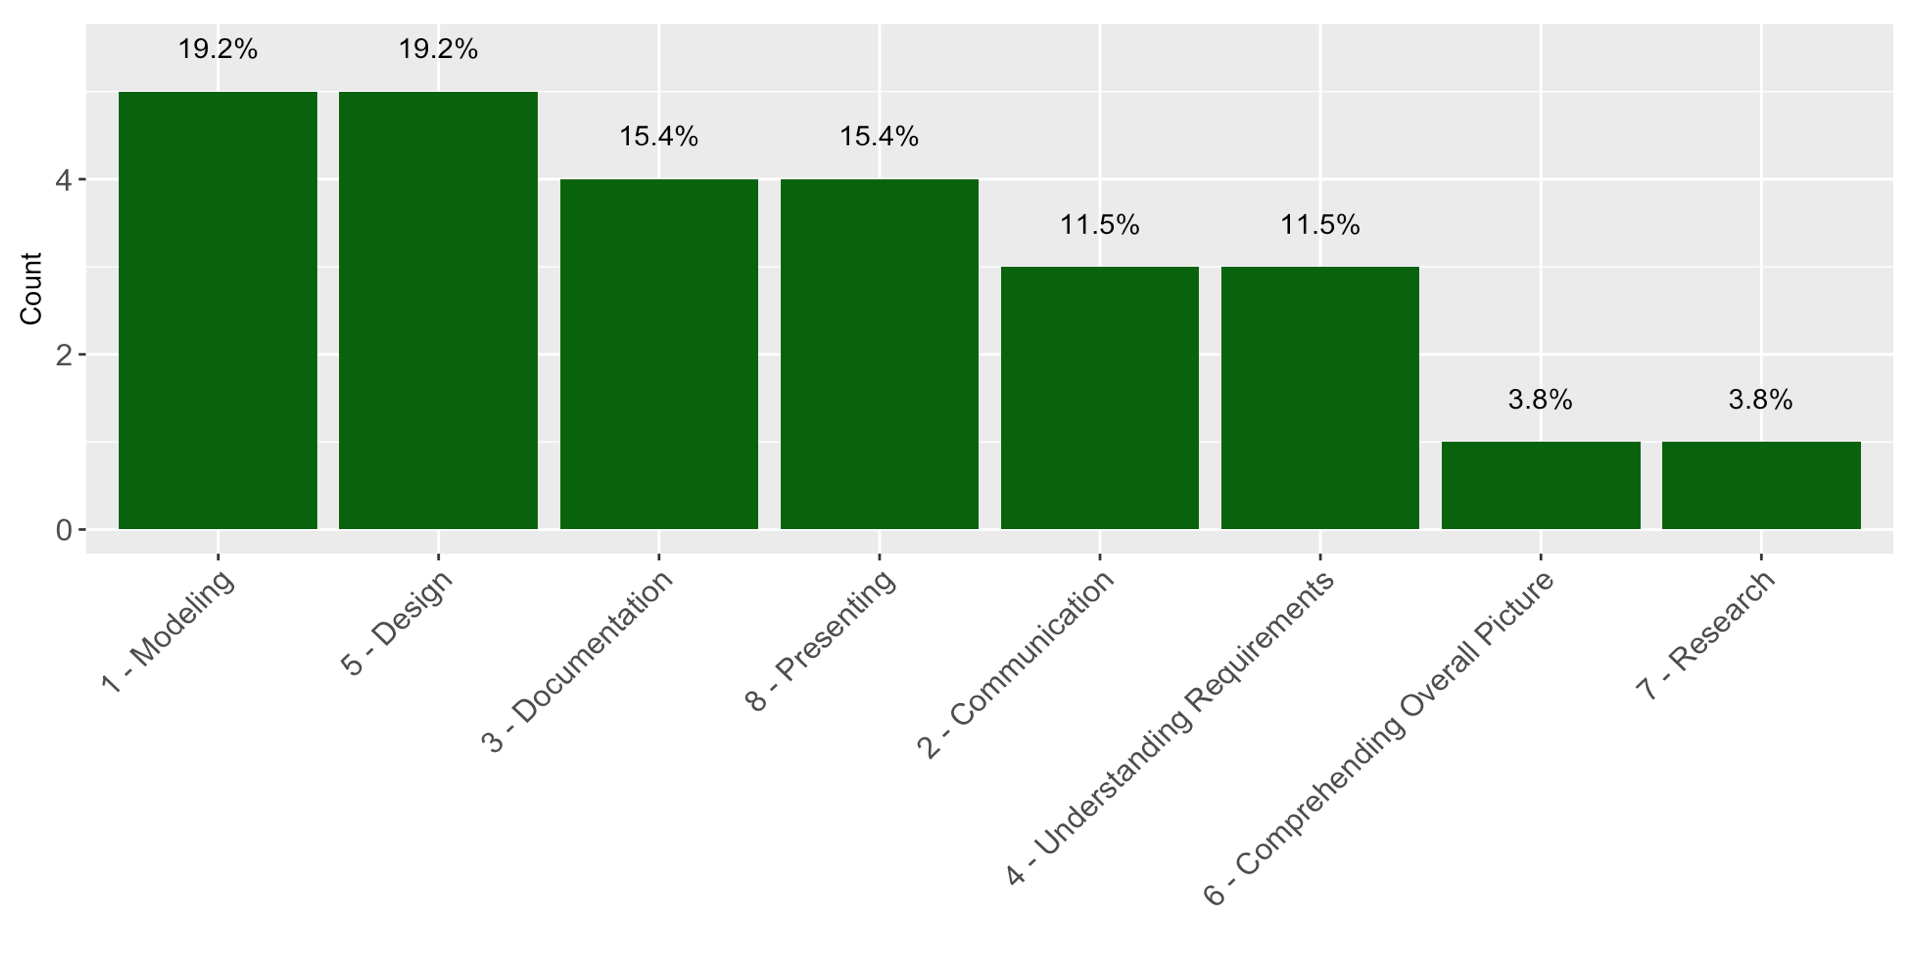
\includegraphics[scale=0.25]{Plots/ActPlot}
      \caption{Software Development Activities involving UML}
      \label{ActUML}
   \end{figure}
   
   
\subsection{RQ4: What are the main issues that hinder the UML use in practice?}

Similar to the question we asked pertaining to the benefits of UML, we also posed an open question asking about the drawbacks of using UML: ``In your opinion, what are the biggest drawbacks of using UML in software development?" We also coded the answers for this question manually. Based on these responses, we came up with 11  codings for the drawbacks of using UML: 1 - High Cost, 2 - Not Universal, 3 - Information Loss, 4 - None, 5 - Security Reasons, 6 - Too Complex, 7 - Maintenance, 8 - Strict Rules, 9 - Time Waster, 10 - Too Formal, 11 - Insufficient. Figure 11 shows the results of this question. The most common responses were 1 - High Cost and 2 - Not Universal, both with 20.8\%, 7 - Maintenance (16.7\%), as well as 6 - Too Complex and 8 - Strict Rules  both with 8.3\% of responses.

	  \begin{figure}[!htb]
      \centering
      \framebox{\parbox{3in}{\textbf{Conclusion of RQ4: } The most common complaint about using UML in software development for our respondents is that there is a high cost involved and it doesn't seem to be universal. Other notable drawbacks include high maintenance, high complexity, and strict rules.
}}
      \label{RQ4Concl}
   \end{figure}
   
\begin{figure}[!htb]
      \centering
      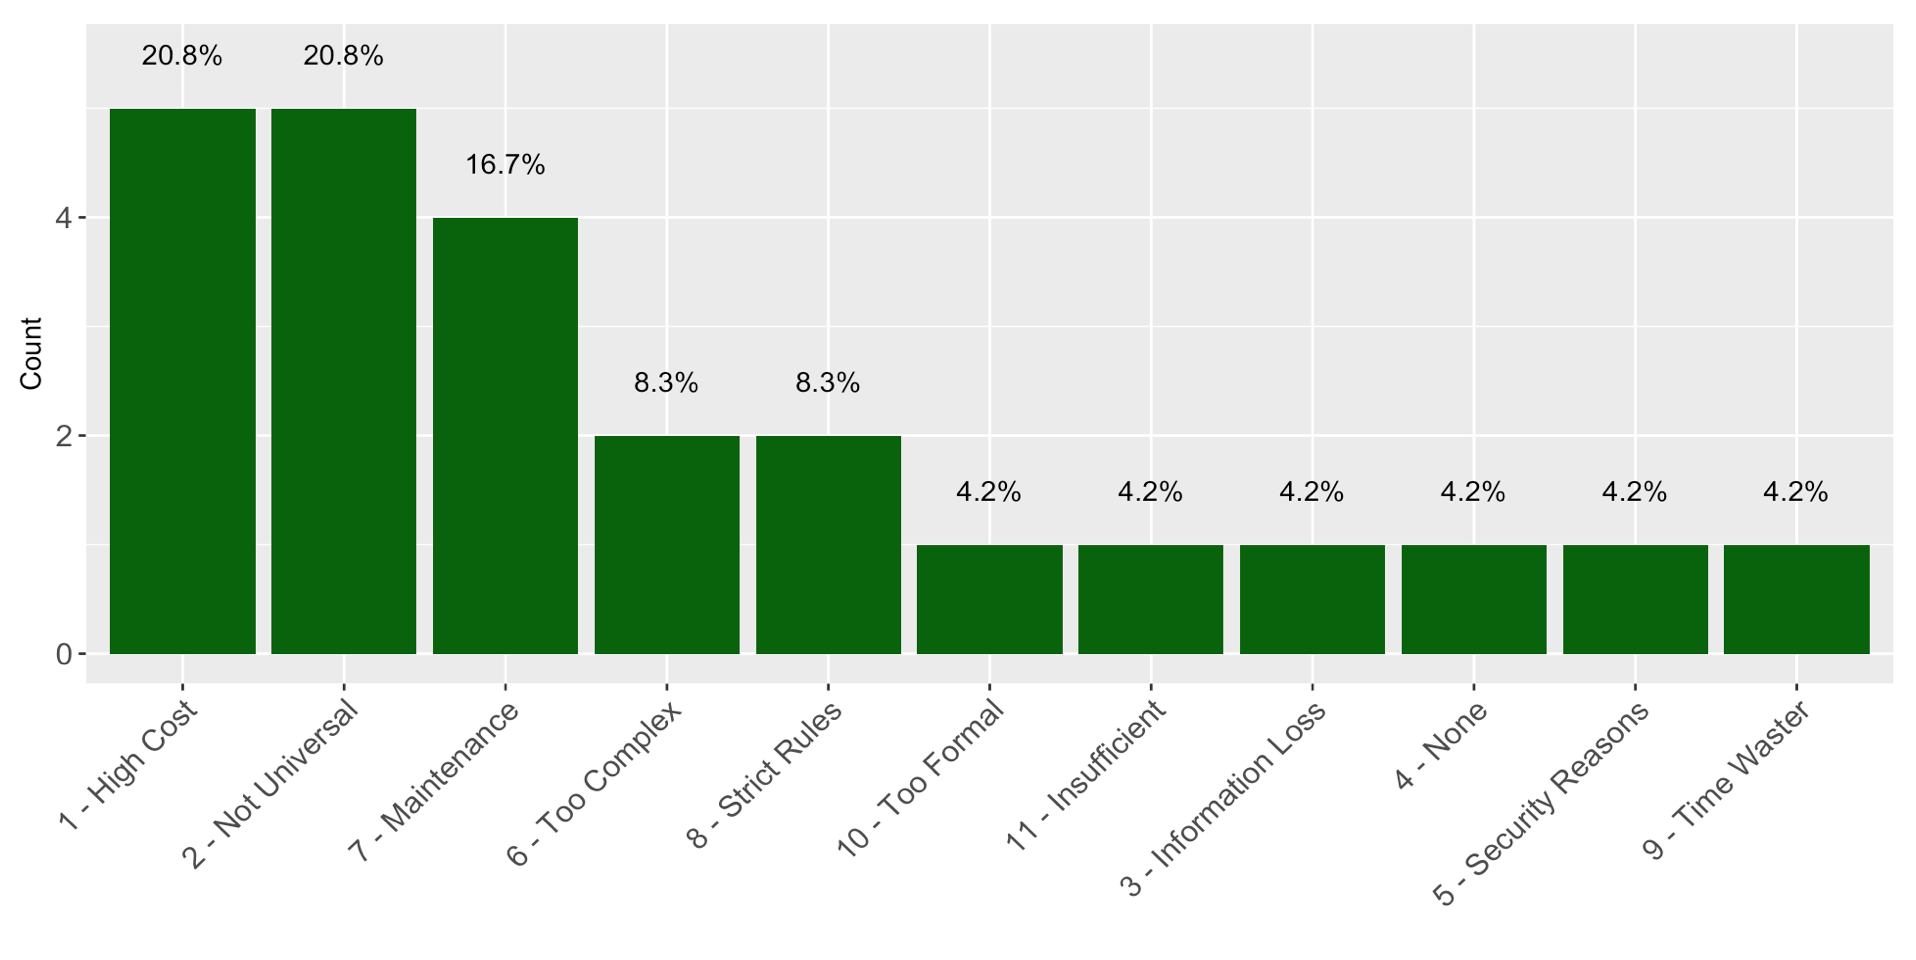
\includegraphics[scale=0.25]{Plots/DrawbacksPlot}
      \caption{Respondent Opinion on the drawbacks of UML usage}
      \label{DrawbUML}
   \end{figure}

\subsection{RQ5: What improvements can be done to increase the UML use?}

This research question was one we wanted to explore specifically in the educational sphere, being where this study originated from. We were particularly interested in whether or not professional Software Engineers believed it worthwhile to educate students in collegiate and other academic programs on the UML use based on their experience in the workplace. Surprisingly, even with the other findings pertaining to our other research questions in the study, every single participant answered ``Yes" to the question of ``Do you think it is important to educate students in collegiate level software engineering programs on the proper use/benefits of UML modeling?"

We also asked participants to optionally provide suggestions on how educational institutions can better educate students in Software Engineering programs on the proper use and benefits of UML through an open question. We manually coded their responses which can be seen in Figure 12 grouped into the following categories: 1 - Hands On Utilization of UML, 2 - Teach in Database Design, 3 - Don't Get Caught Up in Strict Rules, 4 - Emphasize UML is a Common Language, 5 - Interdisciplinary Projects, 6 - Emphasize the Benefits in Early Design, 7 - Continue Teaching Regardless of Popularity, 8 - Don't Overemphasize the Importance. The far most common answer to this question on UML education from respondents was 1 - Hands On Utilization of UML, owning 43.8\% of all answers. The other 7 codings only either received one or two responses. 

	\begin{figure}[!htb]
      \centering
      \framebox{\parbox{3in}{\textbf{Conclusion of RQ5: } The most common suggestion by far from respondents on educating students in academic programs on the proper use and benefits of UML is to give them hands-on experience using UML in their classes for assignments that they are required to complete.
}}
      \label{RQ5Concl}
   \end{figure}
   
\begin{figure}[!htb]
      \centering
      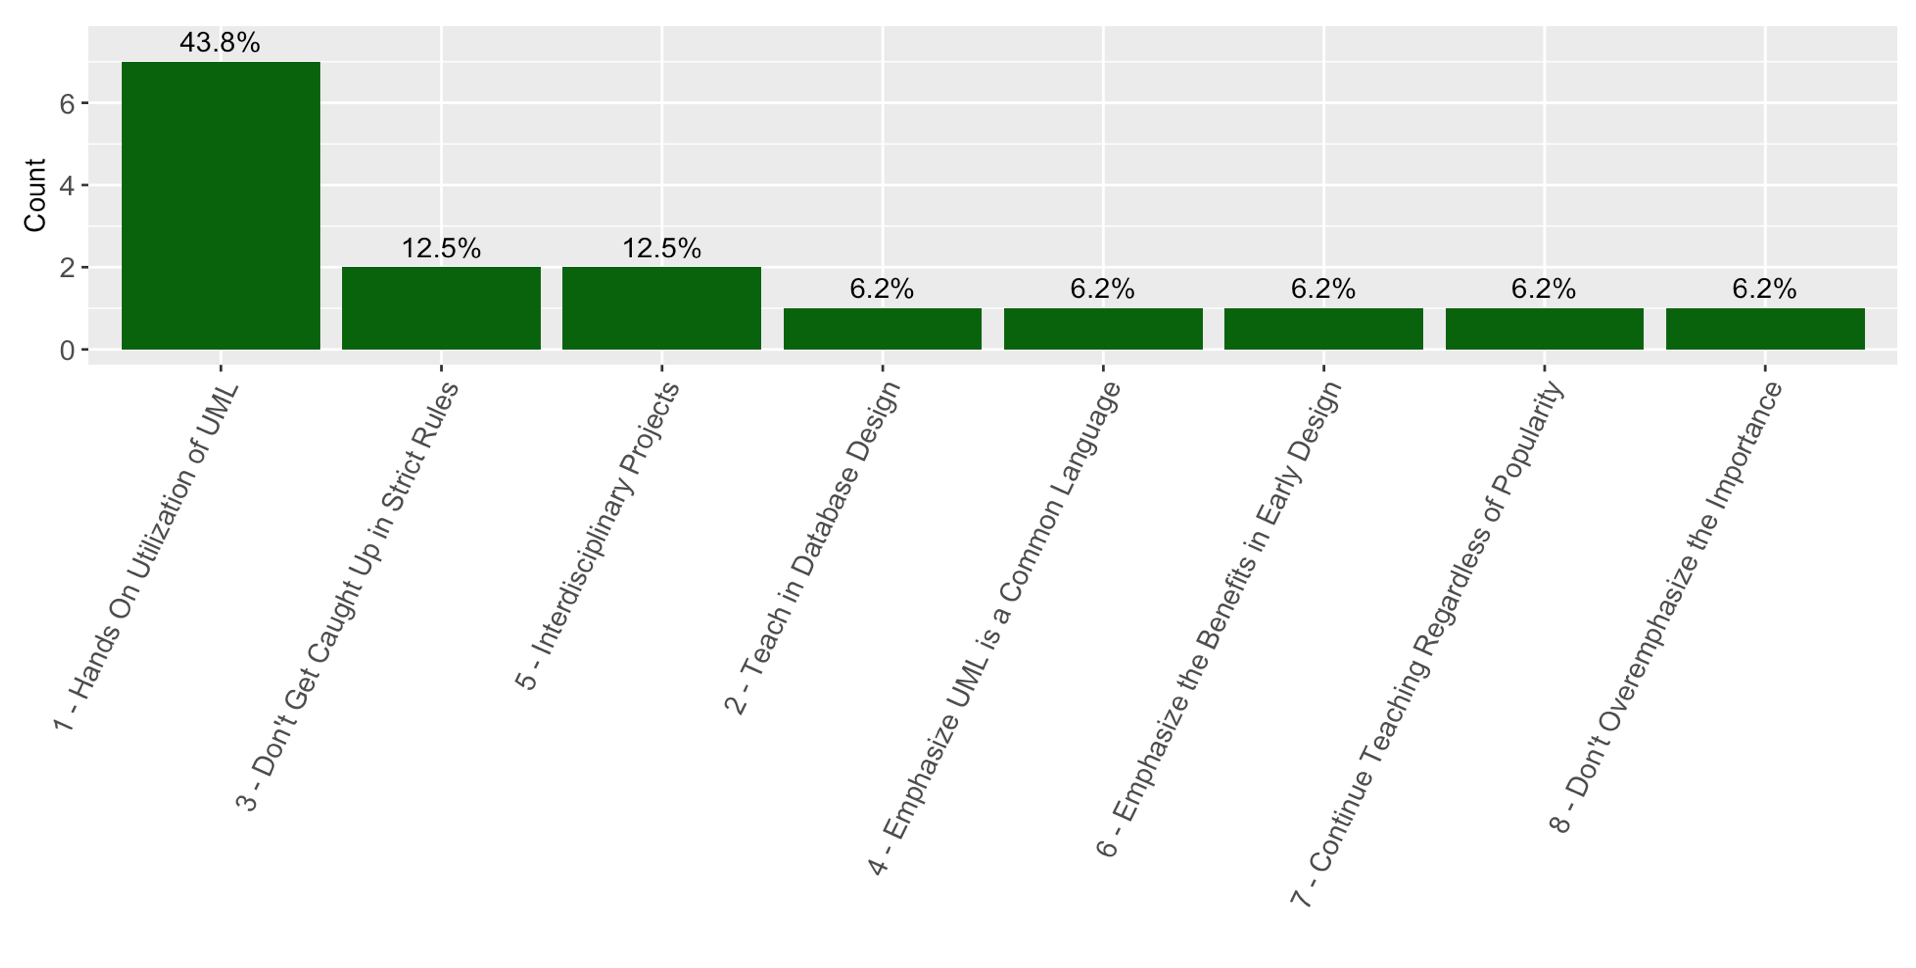
\includegraphics[scale=0.25]{Plots/EduPlot}
      \caption{Respondent Suggestions on Educating Software Engineering Students}
      \label{EduUML}
   \end{figure}
   
\subsection{RQ6: Does project domain influence the use of UML modeling practices?}

As mentioned previously, another potential factor influencing UML usage we were particularly interested in was project domain. Figure 13 shows the distribution of the various organizational domains that our respondents identify with. We allowed them to select more than one in case of any overlap. Over 50\% of our respondents identified their project/organization domain as ``Commercial Software" or ``Technology". Furthermore, Figure 14 breaks down each domain in regards to UML frequency of use in projects individually. It's interesting to note that for all domains with 5 or more responses, the most common response is that participants use UML in 10-50\% of their projects. However, there is simply not enough data to draw any valid conclusions for this research question.

	\begin{figure}[!htb]
      \centering
      \framebox{\parbox{3in}{\textbf{Conclusion of RQ6: } There are some interesting trends in frequency of UML use by Domain, such that in the three main domains for respondents, the leading frequency of UML use is 10-50\%. However, there is not enough data here to look at the other domains and draw any firm conclusions.
}}
      \label{RQ6Concl}
   \end{figure}
   
	\begin{figure}[!htb]
      \centering
      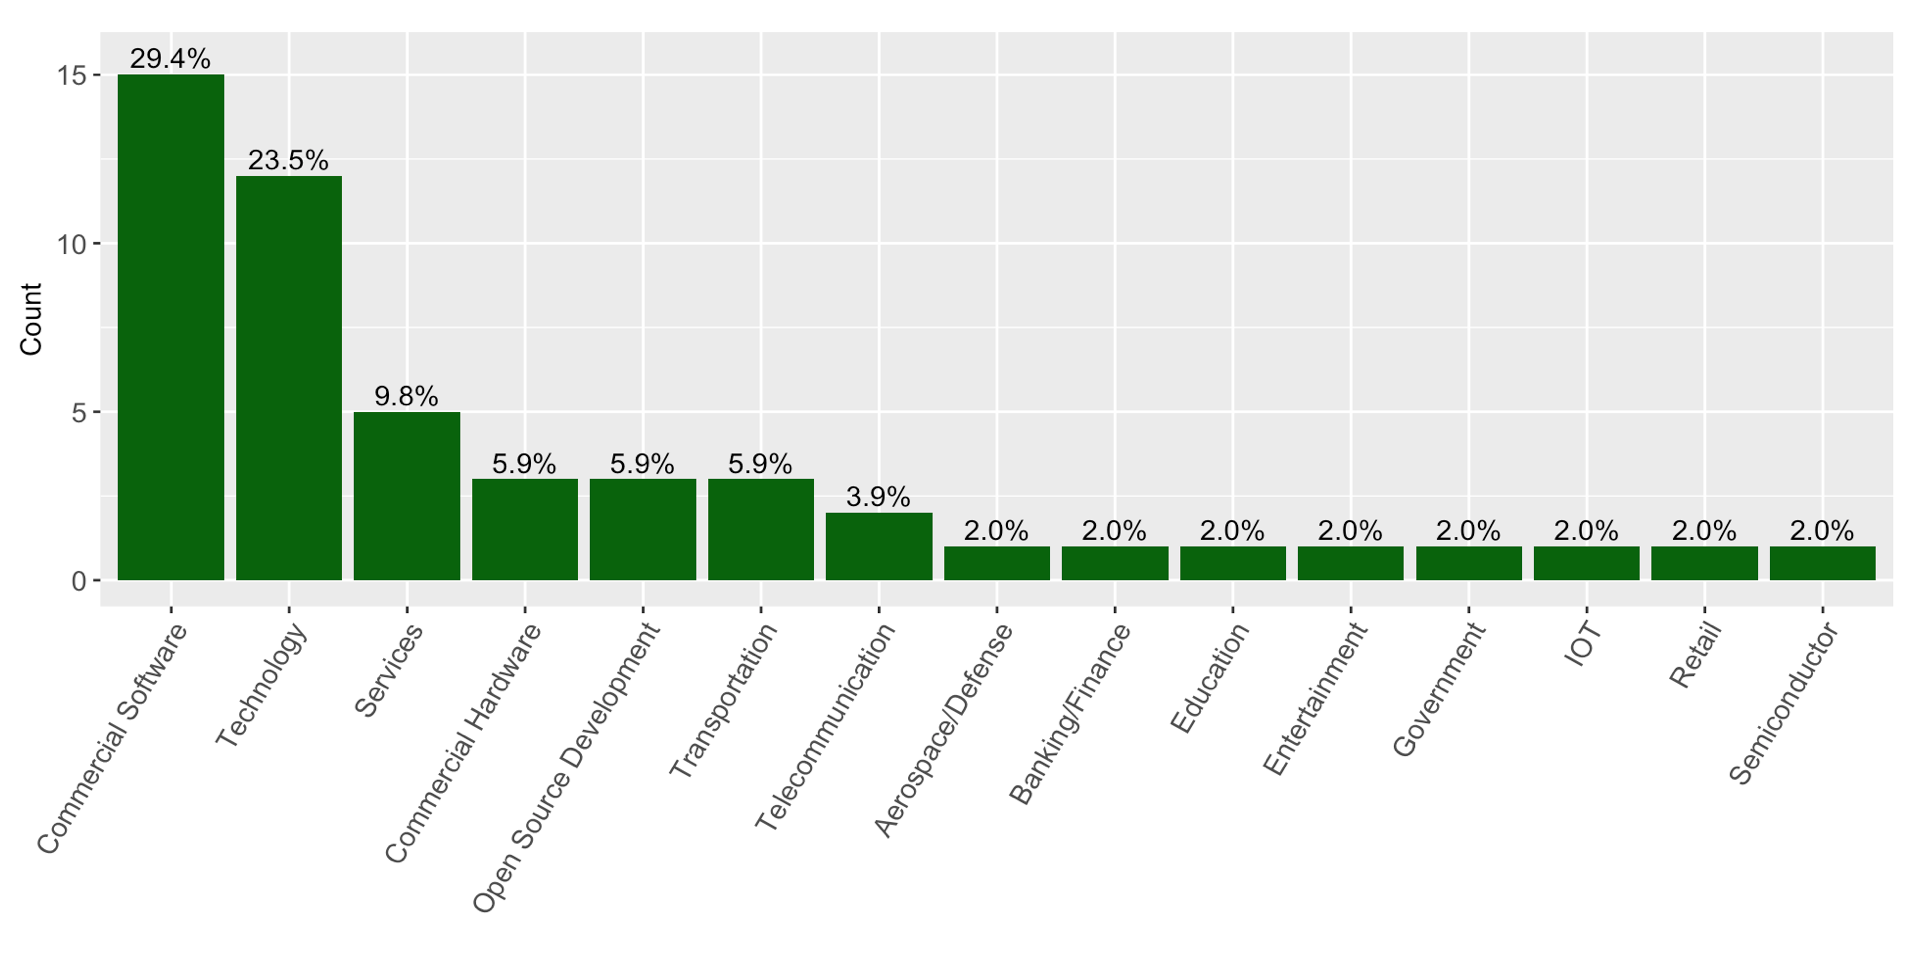
\includegraphics[scale=0.25]{Plots/DomainPlot}
      \caption{Respondent Domain/Industry}
      \label{DomainPlot}
   \end{figure}
   
   \begin{figure}[!htb]
      \centering
      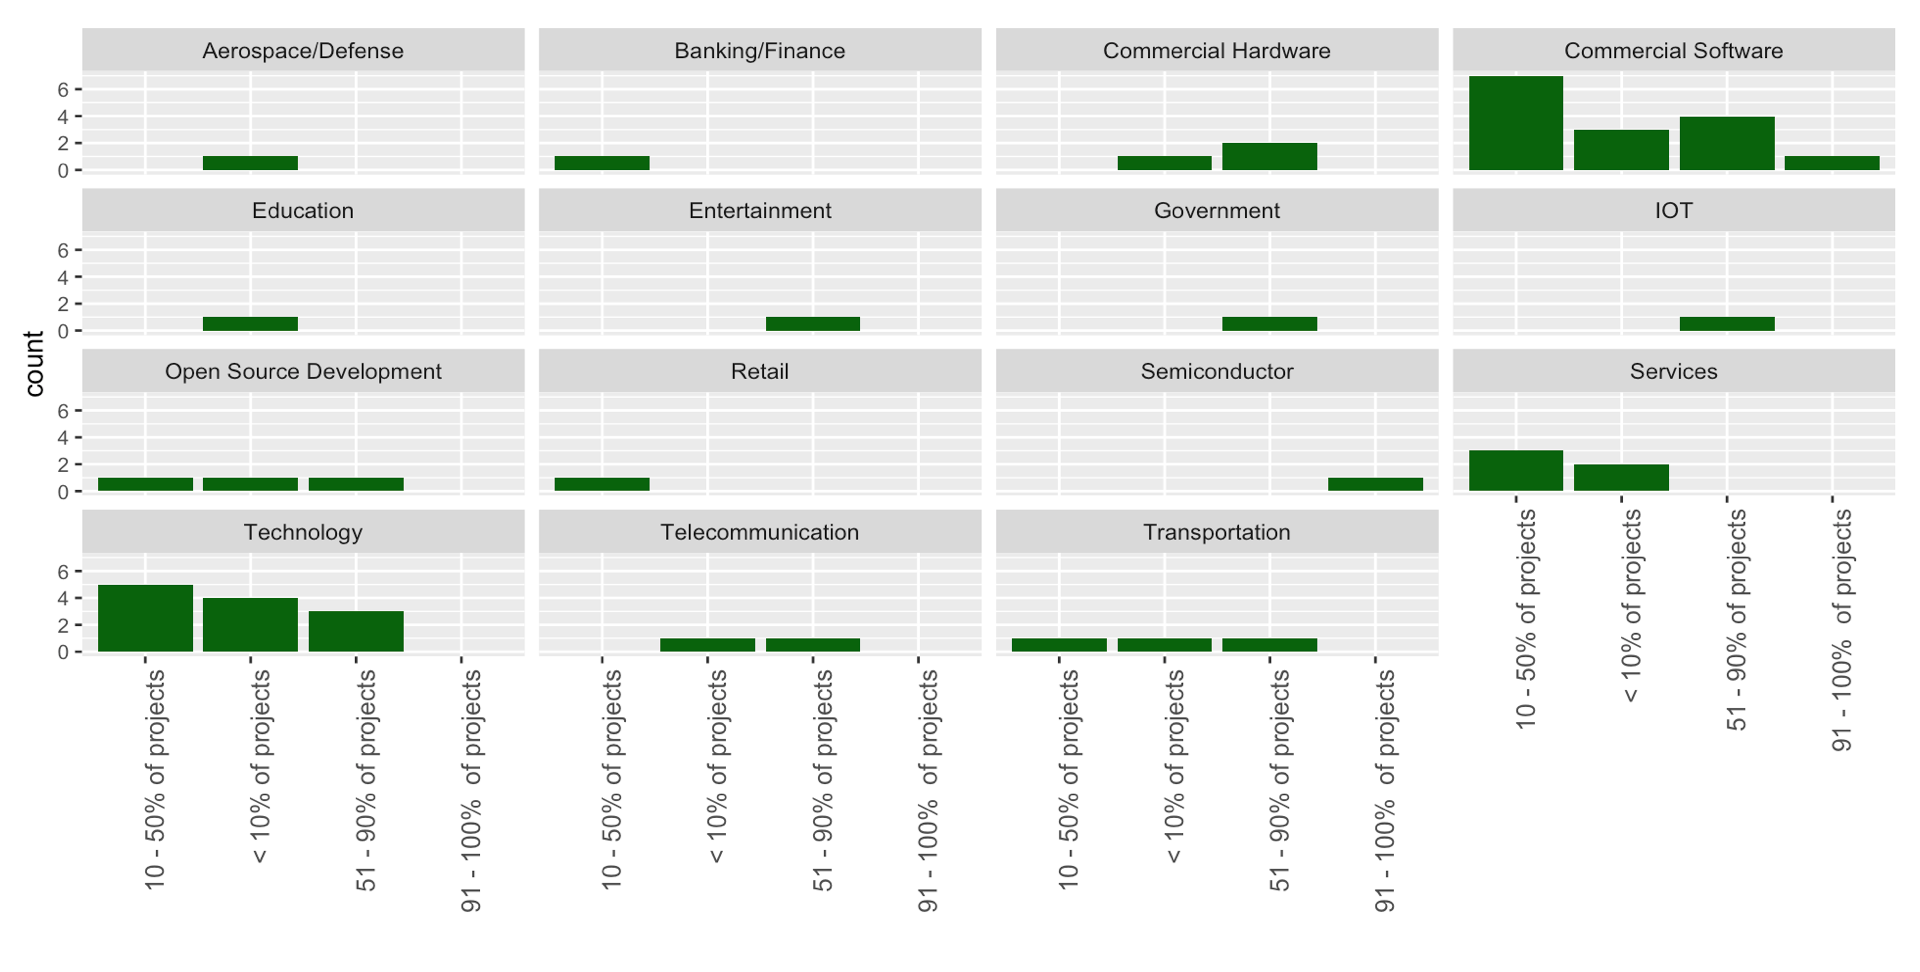
\includegraphics[scale=0.25]{Plots/DomFreqPlot}
      \caption{Respondent Frequency of UML Use by Domain}
      \label{DomFreqPlot}
   \end{figure}

\subsection{RQ7: Does geographic region influence the use of UML modeling practices?}

This research question was not a question we tried to answer with any questions in our survey. Rather, it was the overarching topic of the study, and cannot be answered until the results of this study and further studies on the use and effectiveness of UML in California software industry are compared with studies on UML use and effectiveness in other isolated geographic regions, such as \cite{c3}. Our hope is that this pilot study of UML in California will prompt other researchers in Software Engineering to further examine these topics with many of the same variables, as well as any other additional factors that could potentially affect UML use and effectiveness in specific geographic locations. 


\section{CONCLUSION}

This study surveyed 23 Software Engineers with professional experience in California, with the goal of discovering trends and habits in UML use and opinion on its effectiveness. This was an important question because as Software Engineers, we want to perform at a high level and not be limited by a tool if it is hindering our productivity. The key findings of the study were (1) Average UML use in professional projects falls somewhere between 10 and 90 percent, and there is a disparity among the different kinds of UML diagrams and how often they are used; (2) UML's biggest perceived benefit is its ability to increase communication effectiveness, and has many other perceived benefits on implementation, quality, efficiency, and more; (3) The most common activities respondents utilize UML for are  modeling, design, documentation, presenting, communication, and understanding requirements; (4) UML's biggest perceived drawback is its high cost and lack of universality at times; (5) Respondents suggest that academic institutions educate Software Engineering students on UML by giving them hands on experience in projects. Unfortunately with such a small pool of respondents, it is difficult to say whether or not these conclusions are representative of the entire California software industry. The biggest improvement we feel that could be made to our study and built upon in the future is the way that it is advertised. Finding some way to interact with Software Engineers in person or possibly making the survey handwritten could be potential ideas for increased survey participation. Our hope is that other researchers will continue to examine the California software industry as an extension of this study, as well as many other regions in order to help piece together the picture of UML usage and effectiveness as a whole. 

\addtolength{\textheight}{-12cm}   % This command serves to balance the column lengths
                                  % on the last page of the document manually. It shortens
                                  % the textheight of the last page by a suitable amount.
                                  % This command does not take effect until the next page
                                  % so it should come on the page before the last. Make
                                  % sure that you do not shorten the textheight too much.

%%%%%%%%%%%%%%%%%%%%%%%%%%%%%%%%%%%%%%%%%%%%%%%%%%%%%%%%%%%%%%%%%%%%%%%%%%%%%%%%



%%%%%%%%%%%%%%%%%%%%%%%%%%%%%%%%%%%%%%%%%%%%%%%%%%%%%%%%%%%%%%%%%%%%%%%%%%%%%%%%



%%%%%%%%%%%%%%%%%%%%%%%%%%%%%%%%%%%%%%%%%%%%%%%%%%%%%%%%%%%%%%%%%%%%%%%%%%%%%%%%

\nocite{*}
\bibliography{bibli}
\bibliographystyle{plain}









\end{document}
